\chapter{Multicast Over Resource Limited Sensor Nodes}
\label{chap-tinyadmr}

\section{Introduction}

Publish/subscribe routing is essential to CodeBlue architecture because it
lays the foundation for other core services, including the sensor discovery
layer and the CodeBlue query layer. This chapter presents our experience on
implementing a multicast routing protocol, Adaptive Demand-Driven Multicast
Routing (ADMR)~\cite{admr}, in TinyOS targeting the MicaZ mote platform. MicaZ
platform uses the CC2420 IEEE 802.15.4 radio that is popular among sensor
network research community. We chose ADMR out of three ad-hoc multicast
routing protocols because it achieves the highest performance and require lowest
overhead under high mobility, according to published simulation
studies~\cite{admr, maodv, odmrp}.
To our knowledge, ADMR has never been implemented on
real hardware, although its design has been studied in {\em ns-2} simulations
assuming an IEEE 802.11 MAC.  Our overarching goal is to study the challenges
involved in translating this style of protocol into a real implementation on
wireless sensors. 

Several important lessons have emerged from this experience. The first is
that routing performance is very sensitive to path selection metrics. The ADMR
design attempts to minimize path hop count, but this can result in very lossy
paths~\cite{etx,awoo-multihop}. We describe a new metric that estimates the
overall path delivery ratio with a simple hop-by-hop measurement of the
CC2420's Link Quality Indicator (LQI). The second lesson involves the impact
of protocol overhead and practical limitations on data rates given the very
limited radio bandwidth of IEEE 802.15.4. The third lesson deals with the
impact of limited memory on routing protocol state. We evaluate several
approaches for selectively dropping reverse-path information when the size of
this state exceeds memory availability.

We present a detailed evaluation of our TinyOS implementation of ADMR running
on a 30-node indoor sensor network testbed, MoteLab. MoteLab exhibits a great
deal of variation in link quality and exercises the ADMR protocol in several
ways. We present a comparison of several path selection policies, as well as
demonstrate the impact of varying data rates, interference from other
transmitters, and limitations on routing protocol state. 

\section{Adaptive Demand-Driven Multicast Routing (ADMR)}
\label{sec-tinyadmr-background}
\label{sec-tinyadmr-admr}

\begin{figure}
\begin{center}
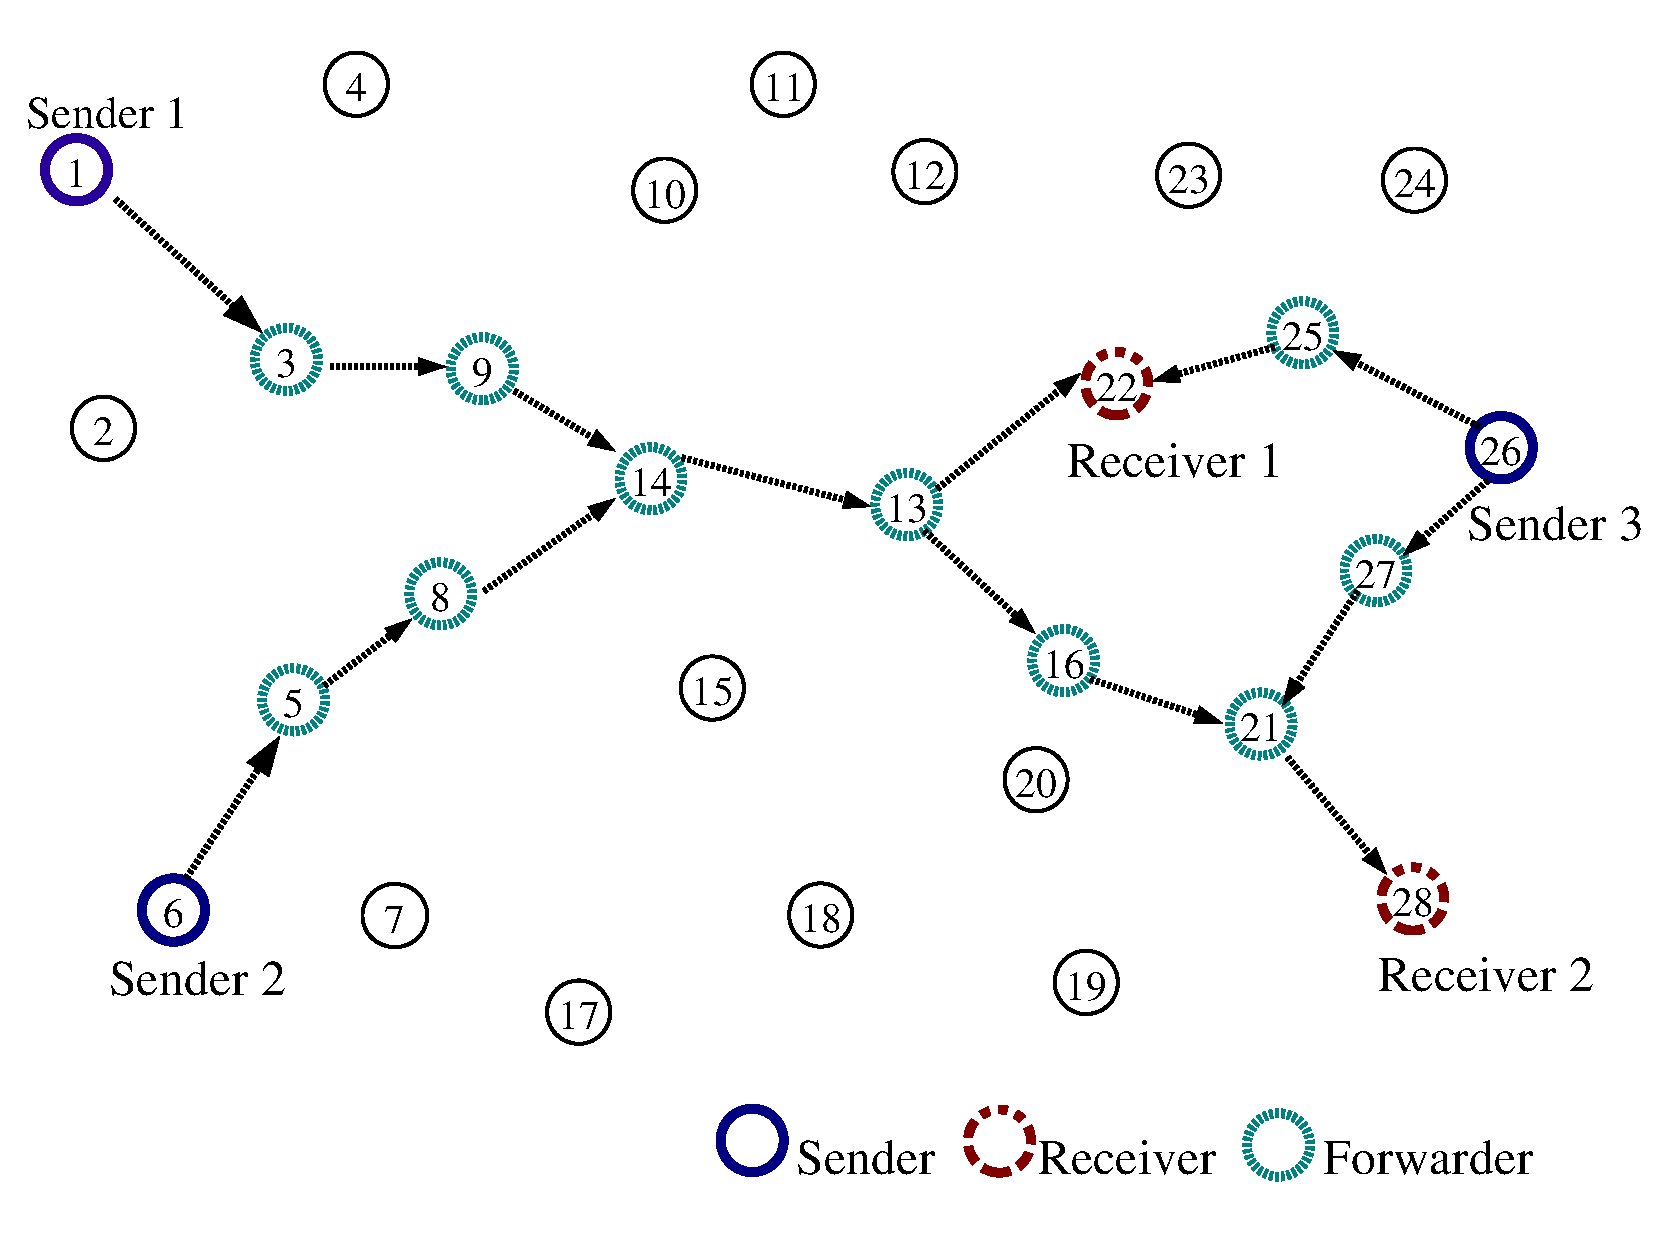
\includegraphics[width=0.6\hsize]{./resources/tinyadmr-techrept05/figures/background/network.pdf}
\end{center}
\caption{{\small {\bf Example of ADMR forwarding trees for a single
group.} {\em Two forwarding trees are established to route data to
the two receiving nodes, 22~and~28. Nodes 1, 6 and 26 are the senders. 
Intermediate nodes act as forwarders, rebroadcasting messages
for the group until they reach the receivers.}}}
\label{fig-network}
\end{figure}

Adaptive Demand-Driven Multicast Routing (ADMR)~\cite{admr} is a
multicast routing protocol designed for ad-hoc networks in which
nodes collaborate with each other to deliver packets. 
Data is multicast by sending packets to {\em group
addresses} rather than individual {\em node addresses}. These packets
will then be forwarded towards all the receivers belonging to a 
particular group along a forwarding tree established by the protocol. 
In this section, we present a brief overview of the ADMR protocol as
designed in~\cite{admr}. 


\subsection{Data packet forwarding}

ADMR delivers packets from senders to receivers by routing each packet
along a set of {\em forwarding trees} that are constructed on demand.
Each tree is rooted at a single receiver and has leaves at each sender
node for a group. ADMR's {\em route discovery} process 
assigns nodes in the network to be {\em forwarders} for a
group based on measurements of potential routing paths 
between senders and receivers. Nodes assigned as forwarders 
rebroadcast data packets received for the corresponding group.

Forwarders are ignorant of the recipients for
any group; rather, they simply rebroadcast group messages, and
a single broadcast may be received by multiple
nodes (including receivers or other forwarders). 
ADMR may also cause messages to traverse multiple routes from
the sender to receiver.
Each ADMR forwarder performs duplicate packet suppression by keeping 
track of the previously-transmitted sequence number for each
$\langle \mathit{sender},\mathit{group} \rangle$ pair; a forwarder
will not rebroadcast the same data packet multiple times.

\begin{figure}
\begin{center}
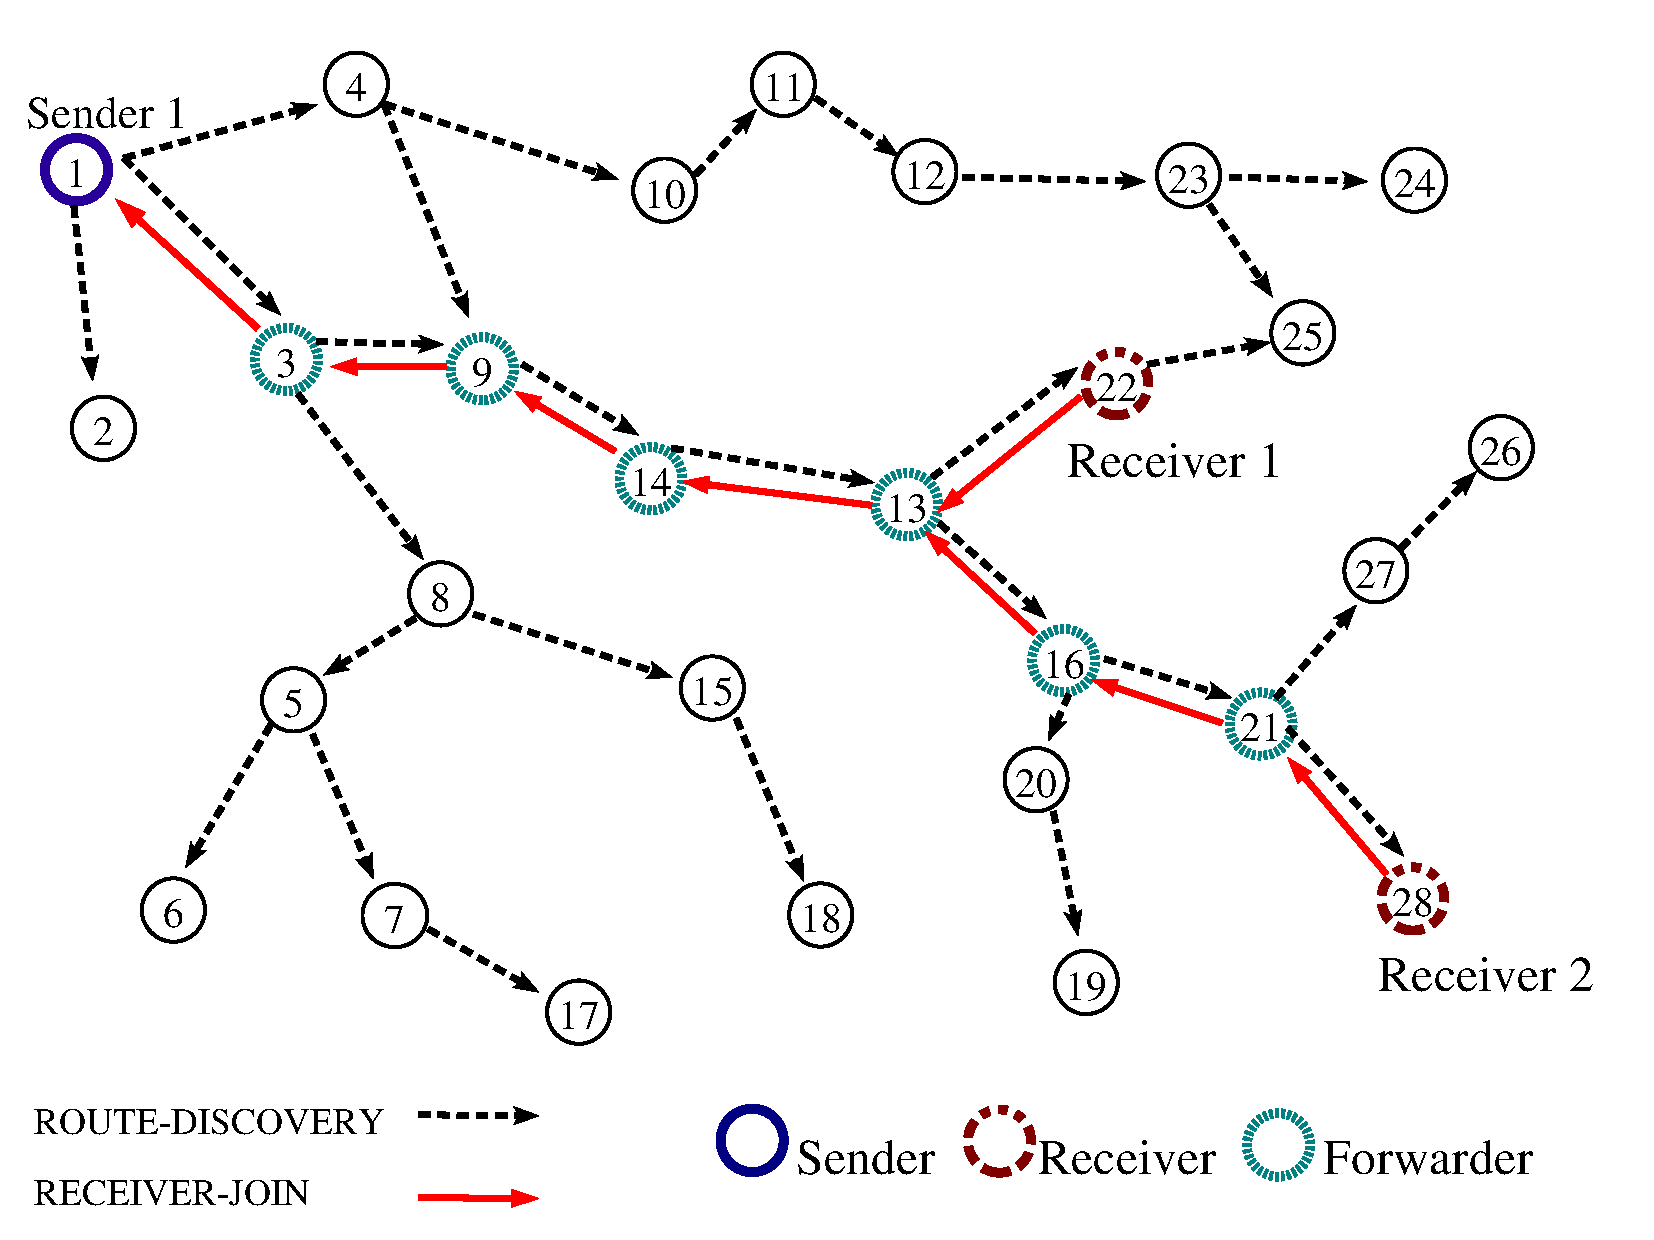
\includegraphics[width=0.6\hsize]{./resources/tinyadmr-techrept05/figures/background/admr_discovery.pdf}
\end{center}
\caption{{\small {\bf The ADMR route discovery process.}
{\em The sender broadcasts a ROUTE-DISCOVERY packet containing a 
group address as a network flood. Receivers for this group
respond with a unicast RECEIVER-JOIN packet, which configures
nodes along the route from the sender as forwarders for the group.}}}
\label{fig-discovery}
\end{figure}

Figure~\ref{fig-network} illustrates an example of ADMR forwarding trees.
In this case, there are 3 senders and 2 receivers in
one group in the network. 10 nodes are selected as forwarders. 
Because both routing trees belong to the same group, there is no
need to transmit data multiple times along links shared between trees; 
the link from node 14~to~13 is an example.

\subsection{Route discovery}
\label{sec-tinyadmr-discovery}

Route discovery is the process of assigning forwarders in the network. 
In the original ADMR design,
there are two ways of establishing forwarding states: 
{\em sender-initiated discovery} and 
{\em receiver-initiated discovery}. In sender-initiated discovery,
senders initiate a network flood to find potential receivers.
Receiver-initiated discovery reverses this process and 
has receivers flooding the network to discover senders.

In the presence of asymmetric radio links, we expect that
sender-initiated discovery will outperform receiver-initiated
discovery. This is because the information propagated through
the network flood is used to measure the routing cost from
senders to receivers, as described in detail below. When this 
process is initiated by sending nodes, the {\em forward path} 
from senders to receivers is measured. Receiver-initiated discovery
measures the {\em reverse path}, which may suffer severe packet 
loss when data packets are forwarded along this route in the 
opposite direction. While we have implemented both discovery
techniques, we only discuss sender-initiated discovery further for brevity.

The route discovery process (Figure~\ref{fig-discovery})
begins with senders sending out a ROUTE-DISCOVERY
packet as a controlled network flood. Every node receiving 
this packet rebroadcasts the packet {\em once} allowing the
message to propagate throughout the network. Upon receipt of
a ROUTE-DISCOVERY message, the node compares the
hop count of the ROUTE-DISCOVERY to the lowest stored
hop count (if any) from the sender generating the discovery. 

If the new hop count is lower, the node stores three
pieces of information: the {\em sender address} that originated the
discovery, the {\em previous hop} from which the discovery message
was received, and new {\em hop count} of the discovery message.
This information is refreshed each time the sender initiates a 
new discovery process, as indicated by a sequence number in 
the message header. In this way, each node maintains the lowest hop 
count path from all sending nodes, as well as the previous hop from 
this sender. 

When a receiver interested in the group specified in the discovery
message receives ROUTE-DISCOVERY, it
sends a RECEIVER-JOIN packet back to the original sender
as a unicast message using path reversal. That is, the
RECEIVER-JOIN is relayed along the lowest hop-count path back to 
the sender, using the stored previous hop information. 
Each intermediate node receiving a RECEIVER-JOIN
configures itself as a {\em forwarder} for the corresponding
$\langle \mathit{sender},\mathit{group} \rangle$ pair.
Once a sender receives any RECEIVER-JOIN, it can start
broadcasting data packets for this group. The forwarding nodes
will relay the messages until they reach the receivers.

Two issues arise with this design. First, the use of
minimum hop count paths is generally not ideal in real wireless
networks, where link quality can vary greatly. Second, using path
reversal to route the RECEIVER-JOIN back to the sender may traverse
a lossy path due to link asymmetry. We discuss both of these issues
and propose solutions in Section~\ref{sec-tinyadmr-routing-metric}.

\subsection{Forwarding state maintenance}

During the course of operation, network conditions may change due to
node failures, radio interference, or node mobility.
These unpredictable changes cause the forwarding states 
to become stale and potentially ineffective at maintaining
reliable routes. Therefore, forwarding state maintenance procedures 
are required to repair or expire inappropriate states in the network. 

\subsubsection{Rediscovery: reestablishing forwarding states}
When network connectivity changes over time, periodically initiating 
the route discovery process is a straightforward but effective way of 
adapting the network to the variations in the link quality. 
The time between rediscovery periods should be set to the longest 
time that the application can tolerate a broken path. Clearly, 
correctly estimating this parameter is difficult and depends on
node mobility and traffic conditions.

\subsubsection{Tree pruning}
Tree pruning allows ADMR to deactivate unnecessary forwarders 
in the network. When a forwarder is no longer effective at
delivering packets to downstream receivers, it should stop
rebroadcasting messages to avoid wasting bandwidth.
Likewise, if a receiver moves away or is no longer interested in 
the data from a certain group, there is no need to forward packets 
to that receiver. ADMR performs state 
expiration using {\em passive acknowledgments}. Whenever a forwarder 
rebroadcasts a packet, it listens for another downstream node to 
retransmit the packet that it just forwarded. 
If the packet is retransmitted by other nodes, then the forwarding 
state will remain valid. Otherwise, the forwarder will deactivate itself
after an expiration period. 

In Section~\ref{sec-tinyadmr-pruning} we discuss the impact of passive
acknowledgments versus active route reinforcement, which requires
a receiver to periodically refresh forwarders with a RECEIVER-JOIN
message.

\subsection{Routing state}
\label{sec-tinyadmr-route-state}
To support the functions described above, ADMR maintains 3 tables 
on each node: the {\em Node Table}, {\em Membership Table}, 
and {\em Sender Table}. 


\begin{description}
\item[Node Table:]
The Node Table is indexed by the sender node address. Each
entry stores the {\em previous hop} and {\em path cost} measured
from ROUTE-DISCOVERY messages received from this sender.
The previous hop is used for routing RECEIVER-JOIN messages
back to the sender to reinforce this route. In the original
ADMR protocol, the path cost was the number of radio hops from
the sender. The previous hop information in a node table entry 
is only updated when a new
message with a lower path cost is received.
The node table essentially determines which intermediate nodes
are used as forwarders on a path from a sender to a receiver.
The node table also stores the {\em sequence number} of the most
recent ROUTE-DISCOVERY message, used to suppress duplicate
retransmissions. The node table therefore must scale with the
size of the network. In Section~\ref{sec-tinyadmr-node-state} we discuss 
the impact of limited memory capacity on maintenance of the
node table.


\item[Membership Table:]
The Membership Table is indexed by group address and sender node
ID and stores information on whether a node is part of a group for
a particular sender ID (as a receiver, forwarder, or both). 
The forwarder flag is set when 
a RECEIVER-JOIN is routed through the node for the corresponding
$\langle \mathit{sender}, \mathit{group} \rangle$ combination.
The reason that both the sender and group address are 
consulted is to prevent messages from being forwarded
back towards a sender from another branch of the routing
tree; for example, in Figure~\ref{fig-network}, we wish to
prevent messages from node~9 being routed back up the tree to
node~8. The receiver flag is set when a node elects to receive
messages for a group. If neither of these flags are set, 
data packets for this group are dropped by the node.

\item[Sender Table:]
The Sender Table stores a list of group addresses for which a node 
is a sender. The table is consulted when the protocol needs to 
perform periodic path rediscovery. In the original ADMR design,
this table also keeps track of the activeness of the group address
and how often the sender should reinforce the paths associated with it.

\end{description}



\section{TinyADMR Implementation}
\label{sec-tinyadmr-impl}

\begin{figure}[t]
\begin{center}
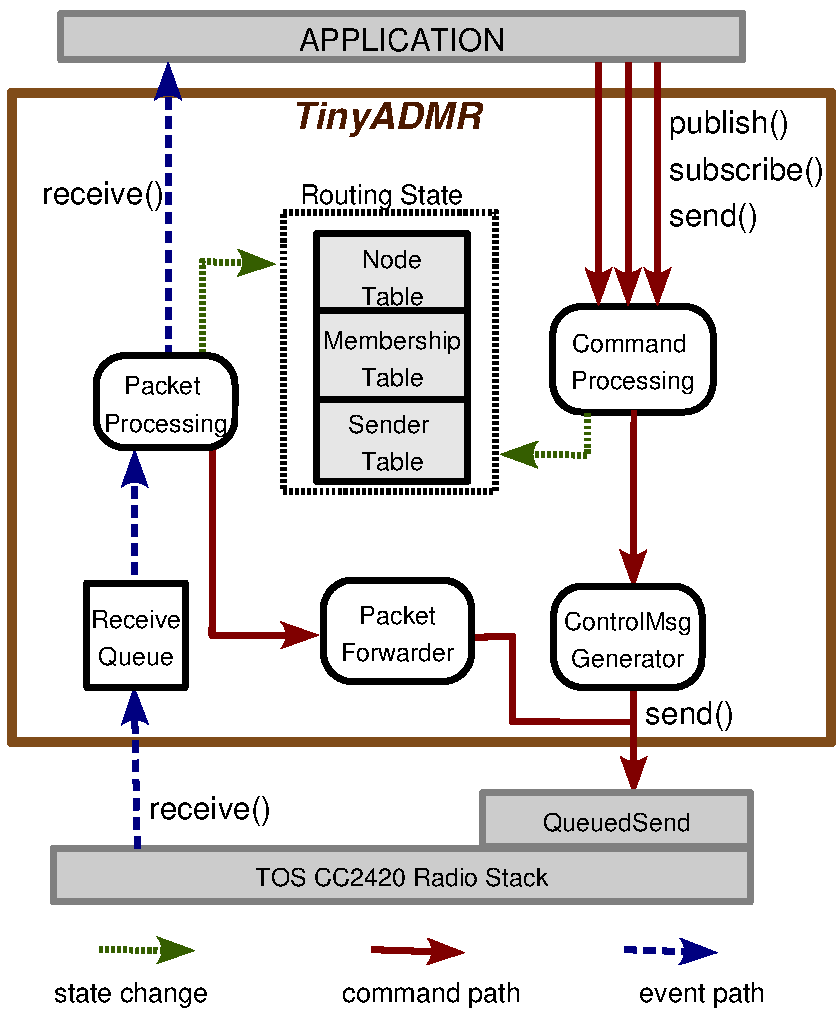
\includegraphics[width=0.6\hsize]{resources/tinyadmr-techrept05/figures/impl/admr_impl_arch.pdf}
\end{center}
\caption{{\small {\bf TinyADMR implementation diagram.}
}}
\label{fig-admrm}
\end{figure}

\begin{figure}[t]
\begin{small}
\begin{verbatim}
interface PubSub {
  command result_t publish(uint16_t chan);
  command result_t subscribe(uint16_t chan);
  command result_t leave(uint16_t chan);

  command result_t send(uint16_t channel, 
      uint8_t length, TOS_Msg* msg);
  event result_t sendDone(TOS_MsgPtr msg, 
      result_t success);

  event TOS_MsgPtr receive(TOS_MsgPtr m, 
      uint16_t channel, uint16_t srcAddr);
}
\end{verbatim}
\end{small}
\caption{{\small\bf The TinyADMR software interface.}}
\label{fig-interface}
\end{figure}

% \begin{figure}
% \begin{footnotesize}
% \begin{verbatim}
% interface PubSub { 
%   command result_t publish(uint16_t groupAddr);
%   command result_t subscribe(uint16_t groupAddr); 
%   command result_t leave(uint16_t groupAddr);
% }
% 
% interface SendMsg { 
%   command result_t send(uint16_t groupAddr, 
%     uint8_t length, TOS_MsgPtr msg);
%   event result_t sendDone(TOS_MsgPtr msg, 
%     result_t success);
% }
% 
% interface ReceiveMsg {
%   event TOS_MsgPtr receive(TOS_MsgPtr m);
% }
% \end{verbatim}
% \end{footnotesize}
% \caption{\small {\bf Interfaces provided by TinyADMR: PubSub, 
% SendMsg and ReceiveMsg.} {\em PubSub supports the Publish/Subscribe 
% membership related functions. SendMsg and ReceiveMsg appear as 
% standard TinyOS SendMsg and ReceiveMsg interface except address
% means group address rather than individual node address.}}
% \label{fig-interface}
% \end{figure}

%  command void* getBuffer(TOS_MsgPtr msg, uint16_t* length);
%  command bool isPublisher(uint16_t groupAddr);
%  command bool isSubscriber(uint16_t groupAddr);


In this section we describe {\em TinyADMR}, our implementation of 
the ADMR protocol for TinyOS-based mote platforms. In developing
TinyADMR, we have attempted to be as faithful as possible to the
original ADMR design. Note that we did not simply port the original 
ADMR code (which was implemented in {\em ns-2}) to TinyOS; this
is a complete reimplementation based on details in~\cite{admr}.
We did consult the ADMR code to understand certain details when 
necessary. Figure~\ref{fig-admrm} depicts the block diagram of 
the TinyADMR implementation. 

TinyADMR deviates from the original ADMR specification in several
respects. First, TinyADMR does not include the sophisticated
route repair protocol described in~\cite{admr}. Instead, we rely on
periodic route rediscovery to refresh routes, which is much simpler. 
As a result, TinyADMR may not be able to respond to a broken route
as rapidly as ADMR. We believe that local route repair is important
in cases where there is both a high degree of node mobility and
a low tolerance for broken routes. In the applications that we
are targeting for ADMR, neither of these conditions hold so we have
not yet implemented this technique.

The most substantial change in TinyADMR is the departure from
hop count as a path selection metric. As we discuss in
Section~\ref{sec-tinyadmr-routing-metric}, we have explored a range of
metrics for picking good paths from senders to receivers.
In TinyADMR, as ROUTE-DISCOVERY messages are propagated through
the network, the code provides a general notion of {\em path cost}
that is stored in the Node Table.

\subsection{Interface} 
\label{sec-tinyadmr-interface}

To provide the applications a clean interface for multicast data 
dissemination, a Publish/Subscribe interface has been defined for 
TinyADMR. The interface is shown in Figure~\ref{fig-interface}.
All communications in TinyADMR are based
on group addresses rather than individual node addresses. Each group
defines a separate communication channel.
Senders send data by publishing to specific group
addresses. Receivers interested in the data subscribe to those group
addresses. The {\tt PubSub} interface is intended to be generic
for supporting any protocol that implements this model.

With TinyADMR, the application expresses its interests in sending
and receiving data on certain group addresses by calling the {\em
PubSub.publish()} and {\em PubSub.subscribe()} commands.
Whenever the application decides to stop participating
on a group address, it calls {\em PubSub.leave()} to cancel its 
membership. The {\em PubSub.send()} command is identical to its TinyOS 
active message counterpart except that it takes a group, 
rather than a node, address as a destination.
{\em PubSub.receive()} event is signaled whenever a data packet arrives
on a group subscribed to by the node. Unlike the regular 
TinyOS {\em ReceiveMsg.receive()} event, {\em PubSub.receive()} provides 
information on both the sender and the group address associated with 
the packet.

\subsection{Protocol implementation}
\label{sec-tinyadmr-impl}

TinyADMR is implemented as a NesC component, {\tt TinyADMR.nc}, 
which wires in several modules providing the protocol functionality.
This component provides the {\tt PubSub} and {\tt StdControl}
interfaces, as well as a separate debugging interface. 
Most of the protocol functionality itself is implemented in 
a single module, {\tt TinyADMRM.nc}, consisting of 1793~lines of
commented NesC code. When compiled for the MicaZ,
TinyADMR requires 3544 bytes of ROM and 1563 bytes of RAM.
Memory usage could be significantly reduced by removing debugging
and instrumentation from the code.

\subsubsection{Packet format}

Each ADMR message carries a 13-byte header, not including the
10-byte header used by TinyOS messages with the CC2420 radio stack.
The header fields are briefly described below:
\begin{description}
\item[{\em pktType}] (one byte): Indicates whether a packet is
a DATA, ROUTE-DISCOVERY, or RECEIVER-JOIN message.
\item[{\em seqNo}] (two bytes): 
Unique sequence number
assigned by the originator of the packet. Nodes that rebroadcast or
forward the packet should not change this field. 
\item[{\em groupAddr}] (two bytes): The group address for the packet.
\item[{\em originAddr}] (two bytes): 
Address of the node that originated the packet. 
\item[{\em senderAddr}] (two bytes): 
Address of the node that last forwarded the packet. 
\item[{\em destAddr}] (two bytes):
Address of the destination node of this packet for unicast messages,
specifically RECEIVER-JOIN. Unused for data and discovery messages.
\item[{\em hopCount}] (one byte):
Number of hops the packet has traversed since
the originator. 
\item[{\em routeCost}] (one byte): 
The accumulated routing cost of a message since it has been originated
by the sender. The meaning of this field varies with the path
selection metric being used.
\end{description}


\subsubsection{Route establishment}

When a node expresses its desire to publish data to a group, 
it invokes {\em PubSub.publish()}, which initiates the periodic
route discovery process. A timer is set that will periodically
issue a flood of ROUTE-DISCOVERY messages from this node. The route
discovery interval is configurable; by default it is set to 15~sec,
although for our experiments in Section~\ref{sec-tinyadmr-lessons} we decreased
the interval to 5~sec to reduce the time to acquire measurements.

Upon receipt of a ROUTE-DISCOVERY message, a node that has 
expressed interest in subscribing to the associated group 
must establish a forwarding path from the sender by 
replying with a unicast RECEIVER-JOIN message. However, reinforcing 
the path taken by the first ROUTE-DISCOVERY message 
will not necessarily yield the best path. Therefore, the receiver
waits for a short time (1~sec in our prototype) in order to acquire
measurements on multiple paths from the sender of the ROUTE-DISCOVERY.  
After this interval, the path with the lowest routing cost (as
indicated by the Node Table entry for the corresponding sender) is
used to relay the RECEIVER-JOIN.

Because RECEIVER-JOIN messages traverse the reverse path from
sender to receiver, in the presence of asymmetric radio links
this message may experience poor links even when the sender-to-receiver
path has high reliability. Therefore, the RECEIVER-JOIN uses
hop-by-hop acknowledgment and retransmission to ensure that it is
routed to the sender. Each node along the path 
attempts to retransmit the RECEIVER-JOIN up to~5~times before 
dropping the message. As a result, it is possible that a very
lossy link will cause the RECEIVER-JOIN to be lost. 
A possible solution is to allow RECEIVER-JOIN messages
to traverse multiple reverse paths and expire redundant forwarders
through tree pruning. 



\subsubsection{Route pruning}

The forwarding tree established for a group during sender and receiver
discovery should be pruned when there are no downstream receivers for
this group or when the sender stops sending data. For this purpose, every 
Node Table entry is assigned a lifetime when it is created.  The 
lifetime of a Node Table entry is decremented by one each time an 
associated timer fires, and the entry is expired when the lifetime becomes 
zero. The lifetime of each entry is refreshed based on a
{\em path reinforcement policy}. 

In TinyADMR, two path reinforcement strategies are implemented:
{\em active reinforcement} and {\em passive reinforcement}. Active
reinforcement refreshes a forwarder membership whenever a new
RECEIVER-JOIN message is received, that is, when a receiver wishes
to keep a node as a forwarder along a path. Passive reinforcement 
refreshes the forwarder membership based on passive acknowledgment of 
each transmitted data packet. 
Details and impact of these two reinforcement methods are discussed
in Section ~\ref{sec-tinyadmr-pruning}.


\subsection{Routing state}

As specified in Section ~\ref{sec-tinyadmr-background}, each node maintains
three tables in order to support the multicast functionality. 
The size of the Node Table depends on how many
nodes are in the network that are acting as multicast senders and receivers.
The size of the Sender and Membership Tables can be determined by 
the number of multicast groups are expected to exist in the network.
Having enough space in the routing tables, especially 
the Node Table, is critical 
because ADMR will not perform properly without large enough table sizes.

The Node Table entries are 8~bytes each. Membership Table entries 
are 7~bytes each, while Sender Table entries are 2~bytes each. By 
default, 
we configure each table to hold 32 entries, resulting in a total
memory use of 544~bytes. In Section~\ref{sec-tinyadmr-node-state} we present
techniques for evicting Node Table entries when memory is limited.


\section{Evaluation and Lessons Learned}
\label{sec-tinyadmr-lessons}

Implementing ADMR in TinyOS and obtaining good communication performance 
in a realistic network environment has not been a trivial undertaking. 
There is a significant disconnect between the original ADMR protocol
as published and the conditions encountered in a real sensor network.
In particular, ADMR assumes symmetric links, uses hop count as
its path selection metric, and ignores memory space issues when
maintaining routing tables. In this section we present a detailed
evaluation of our TinyOS-based ADMR implementation and present a
series of lessons learned in the process of developing and tuning the
protocol. We believe these lessons will be useful to other protocol
designers working with 802.15.4-based sensor motes.

\subsection{Evaluation environment}

We have focused exclusively on real implementation and evaluation on a
sensor node testbed, rather than simulations, to understand the
performance and behavior of TinyADMR. All of our results have been
gathered on an indoor testbed of 30~MicaZ motes installed over three
floors of our Computer Science building (a map of one floor is shown
in Figure~\ref{fig-motelab}). This testbed provides facilities 
for remote reprogramming of each node over an Ethernet back-channel 
board (the Crossbow MIB600). Each node's serial port is also 
exposed through a TCP port permitting detailed instrumentation and debugging.
Motes are installed in various offices and labs and are often placed 
on shelves at a height of 1-2~m. 

\begin{figure*}[t]
\begin{center}
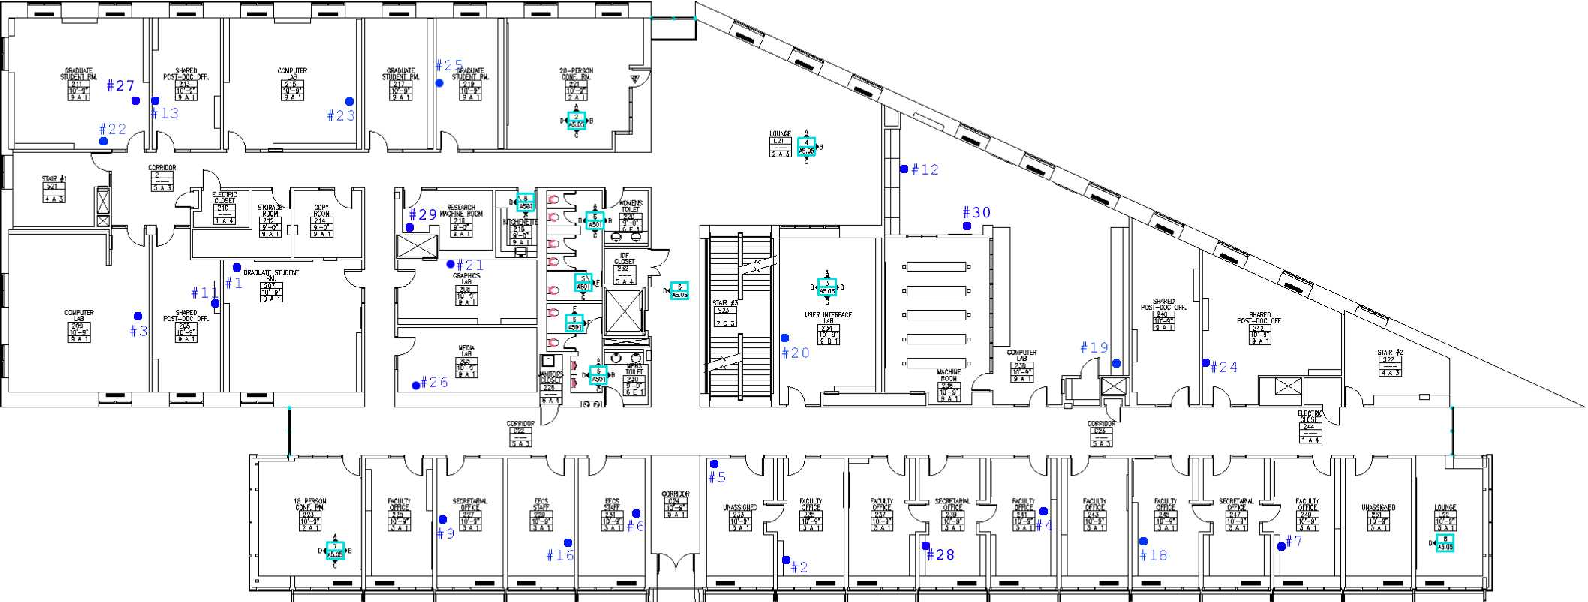
\includegraphics[width=0.9\hsize]{resources/tinyadmr-techrept05/figures/maps/MD-2.pdf}
\end{center}
\caption{{\small {\bf Map of one floor of our 30-node sensor network testbed.}}}
\label{fig-motelab}
\end{figure*}

\begin{figure}[t]
\begin{center}
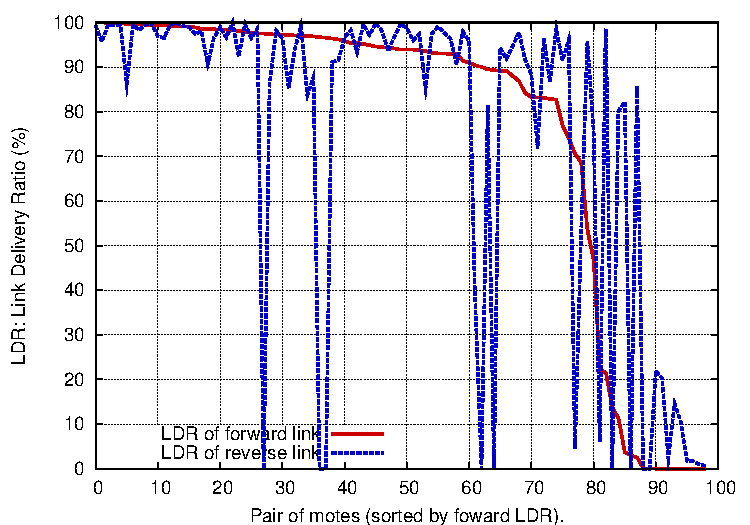
\includegraphics[width=0.6\hsize]{resources/tinyadmr-techrept05/figures/lessons/lqi/link_asymmetry_dr.pdf}
\end{center}
\caption{{\small {\bf Link delivery ratio (LDR) asymmetry observed in
our testbed.}}}
\label{fig-link-asymmetry-dr}
\end{figure}

\begin{figure}[t]
\begin{center}
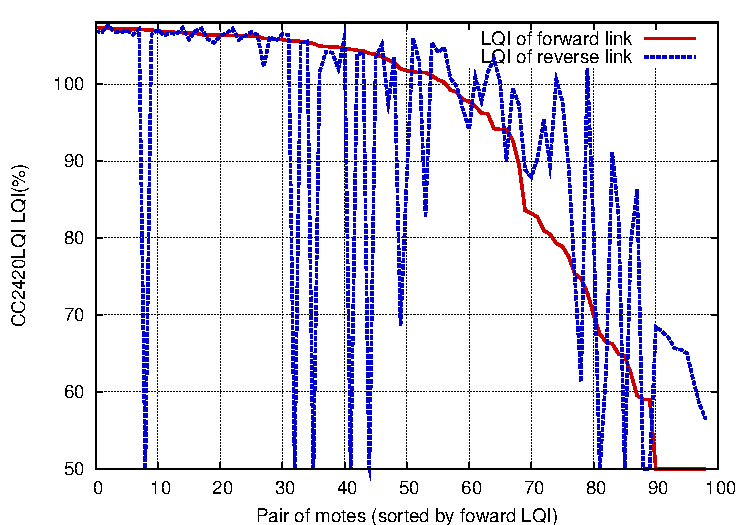
\includegraphics[width=0.6\hsize]{resources/tinyadmr-techrept05/figures/lessons/lqi/link_asymmetry_lqi.pdf}
\end{center}
\caption{{\small {\bf Link-level LQI asymmetry observed in our testbed.}}}
\label{fig-link-asymmetry-lqi}
\end{figure}

\begin{figure}[t]
\begin{center}
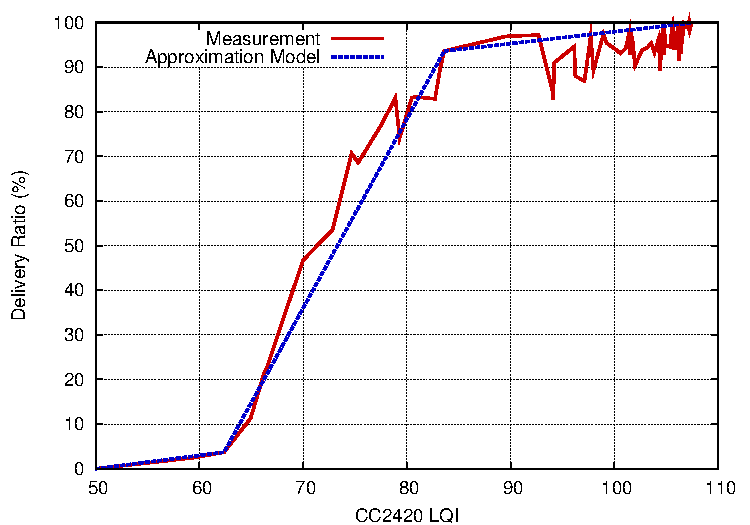
\includegraphics[width=0.6\hsize]{resources/tinyadmr-techrept05/figures/lessons/lqi/dr_vs_lqi.pdf}
\end{center}
\caption{{\small {\bf Relationship between LQI and delivery ratio in our
testbed.}} {\em Also shown is the piecewise linear model used to 
map LQI observations to LDR estimates.}}
\label{fig-del-vs-lqi}
\end{figure}

Because of the relatively sparse node placement, this testbed exhibits
a high degree of variation in radio link quality and many asymmetric
links. Figure~\ref{fig-link-asymmetry-dr} shows the forward and
reverse {\em link delivery ratio} (LDR) calculated for every pair of
nodes in the testbed. Using a technique similar to the
SCALE benchmark~\cite{scale}, the link delivery ratio is measured by 
having each node broadcast a fixed number of messages in turn, while
all other nodes record the number of messages received from each
transmitter. The LDR is the ratio of received messages to transmitted
messages for each pair of nodes. As the figure shows, the LDR is
highly variable and often asymmetric. 

The CC2420 radio provides an internal Link Quality Indicator (LQI)
for each received message~\cite{cc2420-manual}. This value represents
the ability of the CC2420 to correlate the first eight 32-chip symbols
following the start-of-frame delimiter, 
and has an effective range from 110 (highest quality) 
to 50 (lowest quality). As we will discuss in
Section~\ref{sec-tinyadmr-routing-metric}, the LQI is highly correlated with
the link delivery ratio. Figure~\ref{fig-link-asymmetry-lqi} shows
the corresponding asymmetry in the pairwise LQI measurement (averaged
over 1000 packets per transmitter). 

In each of the cases presented below, we measure routes between
28~different sender/receiver pairs. These pairs were selected to present
a diverse view of potential routes in our testbed. Four of the
28~pairs were within a single radio hop, 11~were within two radio
hops, and the remaining 13~pairs were chosen so that the endpoints
were on opposite ends of the building (shown in
Figure~\ref{fig-motelab}). In each case, senders generated
data at a rate of 5~Hz, each experiment was run for~100~sec, 
and path discovery messages were generated every 5~sec.
Once the benchmark is started, we wait for 30~seconds before
collecting packet reception statistics, to avoid measuring
warm-up effects. 

\paragraph*{Original ADMR evaluation:} It is worth contrasting our
environment to that used in the original ADMR paper. 
In~\cite{admr}, ADMR was measured using {\em ns-2} simulations
with a network of 50~nodes roaming in a 1500~m $\times$ 300~m area. 
A 2~Mbps 802.11 radio with a radio range of 250~m was simulated; 
this implies that most nodes are within a small
number of hops of each other. Most importantly, nodes have perfect
connectivity to all other nodes within this range and links are
always symmetric.

\subsection{Impact of path selection metrics}
\label{sec-tinyadmr-routing-metric}

Ad-hoc routing protocols use a {\em path selection metric} to 
determine which path to maintain between a given sender and receiver
pair. In ADMR, the path cost is updated as discovery messages
propagate from senders to receivers. The receiver sends a 
route reply message along the reverse of the lowest-cost path,
which configures nodes along that path as forwarders.

The original ADMR protocol selects paths with the {\em minimum hop
count}, which we call the MIN-HOP metric.
As has been discussed elsewhere~\cite{etx,awoo-multihop},
this choice of metric is not necessarily ideal, especially when 
link quality varies considerably. For example, MIN-HOP will prefer 
a short path over (potentially) very poor radio links rather than
a longer path over high-quality links.  MIN-HOP was appropriate in the
original ADMR work which did not consider lossy radio links. However,
in a realistic environment we expect it to have very poor performance.

\subsubsection{MAX-LQI and PATH-DR metrics}

We have investigated two alternate path selection metrics in our
development of TinyADMR. 
The first is to select the path with the ``best worst link.''
In this metric the receiver selects the path with the highest 
{\em minimum} LQI value over all links in the path. Given a set 
of potential paths $P$ and set of links $L_p$ for each $p \in P$, 
we select the path $p^\star$:
\[
  p^\star = \arg \max_{p \in P} \min_{l \in L_p} \mathrm{LQI}(l)
\]
We call this metric MAX-LQI.

MAX-LQI attempts to find the path with the best ``bottleneck,''
however, it does not have any way of differentiating between
two paths with the same bottleneck link but different 
link characteristics. Because our goal in ADMR is to maximize
the overall {\em path delivery ratio} (PDR), directly
using the path with the best PDR would be ideal. However, estimating PDR
requires measuring the hop-by-hop LDR along the path.
This requires multiple rounds of message exchange between
neighboring nodes, incurring additional messaging overhead.
The ETX~\cite{etx} and MintRoute~\cite{awoo-multihop} protocols
use this technique.

Rather than directly measure LDR, we have found that there is a 
high correlation between the LQI and LDR observed on each link.
Figure~\ref{fig-del-vs-lqi} plots the pairwise LQI and LDR over an
extensive set of measurements in our testbed. 
From this data we can derive a simple {\em model} mapping
LQI to LDR; a piecewise linear approximation appears to work well
for this data set. Because LQI can be observed from a {\em single
packet reception}, using this information to predict the previous-hop
LDR allows us to produce the PATH-DR metric, which selects the
path $p^\star$ such that:
\[
  p^\star = \arg \max_{p \in P} \prod_{l \in L_p} \mathrm{ESTLDR}(l)
\]
where $\mathrm{ESTLDR}(l)$ is the estimated LDR of the link from
the LQI of the received discovery message, derived from our empirical
model shown in Figure~\ref{fig-del-vs-lqi}.

\subsubsection{Results}

\begin{figure}[t]
\begin{center}
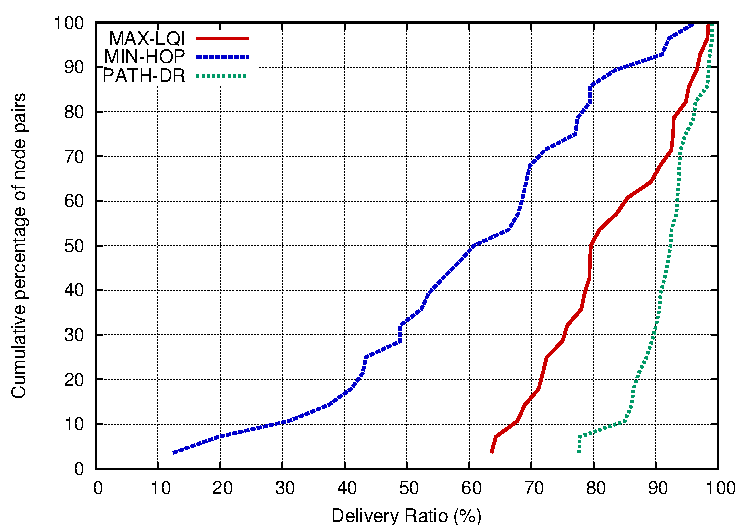
\includegraphics[width=0.6\hsize]{resources/tinyadmr-techrept05/figures/lessons/lqivshop/lqi-hop-pathdr-cdf.pdf}
\end{center}
\caption{{\small {\bf Comparison of MIN-HOP, MAX-LQI, and PATH-DR
routing metrics.} {\em This CDF shows the path delivery ratio measured
over 28~separate pairs of nodes using each of the three metrics.
PATH-DR produces the best results with 50\% of the paths obtaining a
delivery ratio of over 92.4\%.}}}
\label{fig-lqi-hop-pathdr}
\end{figure}

\begin{figure}[t]
\begin{center}
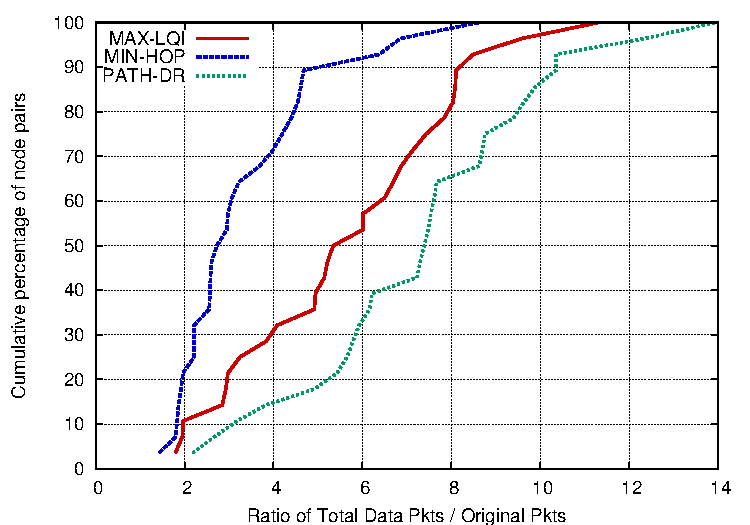
\includegraphics[width=0.6\hsize]{resources/tinyadmr-techrept05/figures/lessons/lqivshop/lqi-hop-pathdr-cdf-oh.pdf}
\end{center}
\caption{{\small {\bf Overhead incurred by each path selection
metric.} {\em This CDF shows the ratio of the number of 
data packets transmitted in the network (including forwarded messages)
to the number of data packets originated by each sender. 
For example, for 70\% of the 28~paths, MAX-LQI resulted in an
overhead of 6~transmissions for every original packet.}}}
\label{fig-overhead}
\end{figure}

\begin{figure}[t]
\begin{center}
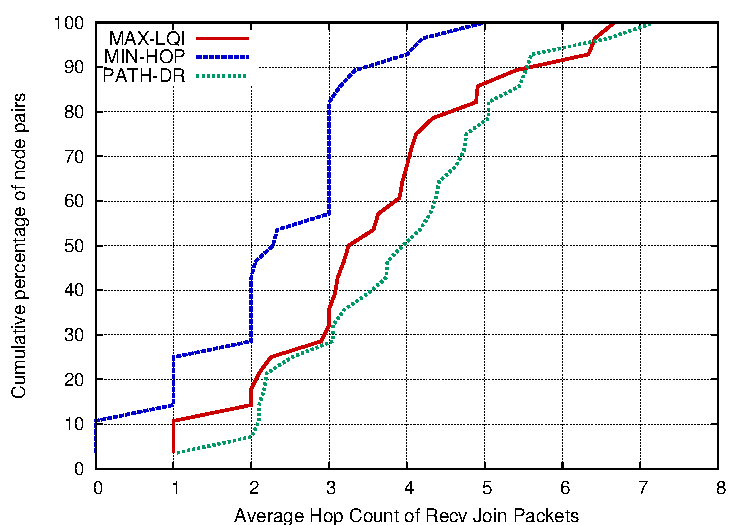
\includegraphics[width=0.6\hsize]{resources/tinyadmr-techrept05/figures/lessons/lqivshop/lqi-hop-pathdr-cdf-rcv.pdf}
\end{center}
\caption{{\small {\bf Path lengths for receiver join messages for each
path selection metric.} {\em This CDF shows the length of
the paths selected by receivers for each metric. The MIN-HOP metric
minimizes the hop count, while MAX-LQI and PATH-DR incur some path
stretch because they focus on higher-quality links.}}}
\label{fig-pathlength}
\end{figure}

\begin{figure}[t]
\begin{center}
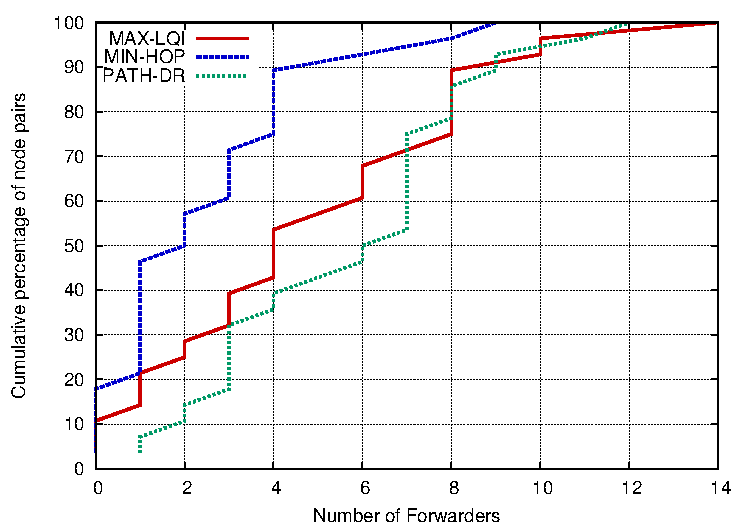
\includegraphics[width=0.6\hsize]{resources/tinyadmr-techrept05/figures/lessons/lqivshop/lqi-hop-pathdr-cdf-fwd.pdf}
\end{center}
\caption{{\small {\bf Number of active forwarders for each path
selection metric.} {\em This CDF shows the number of forwarders that
are active while routing data for each of the 28~paths. The number of
forwarders is not identical to the path length in 
Figure~\ref{fig-pathlength} because
multiple paths may be active.}}}
\label{fig-num-forwarders}
\end{figure}


Figure~\ref{fig-lqi-hop-pathdr} shows a CDF of the path delivery ratio
for the set of 28~paths. As the figure shows, PATH-DR results in the
highest delivery ratio over all paths, with nearly all paths resulting
in a PDR of over 80\%, and a median of 92.4\%. MAX-LQI also performs
well, with a median PDR of 79.6\%. MIN-HOP is noticeably worse, with a
median PDR of just 60.7\%.

PATH-DR and MAX-LQI achieve higher robustness at the cost of
higher overhead. In addition to taking longer routes, 
multiple routing paths may be active between a sender and
receiver at once. The existence of multipath routes should
result in higher path delivery ratios. Figure~\ref{fig-overhead} shows
the overhead for each path selection metric 
in terms of the ratio between the total number of transmitted
messages and the number of messages generated by each sender.
This ratio is at least as high as the number of routing hops from
sender to receiver, and will be higher when multiple routes are involved. 

The path length for each receiver join message is shown in 
Figure~\ref{fig-pathlength}, while the total number of active
forwarders for each node pair is shown in Figure~\ref{fig-num-forwarders}.
The median path length for MIN-HOP is 2~hops, where it is about 
4~hops for both PATH-DR and MAX-LQI.
The number of forwarders is somewhat higher than the number of hops
because PATH-DR and MAX-LQI may activate multiple paths on 
subsequent route selection phases. The impact of pruning these
extra routes is presented in Section~\ref{sec-tinyadmr-pruning}.

These results show that the routing selection metric has a
large impact on performance and communication overhead. 
The PATH-DR metric provides high reliability using a simple
model mapping the CC2420's LQI to LDR, making it straightforward
to implement without incurring additional measurement overhead.
We can imagine a wide range of alternate path selection metrics 
as part of future work.

\subsubsection{Stability of path measurements}

\begin{figure}
  \begin{center}
    \begin{tabular}{c}
      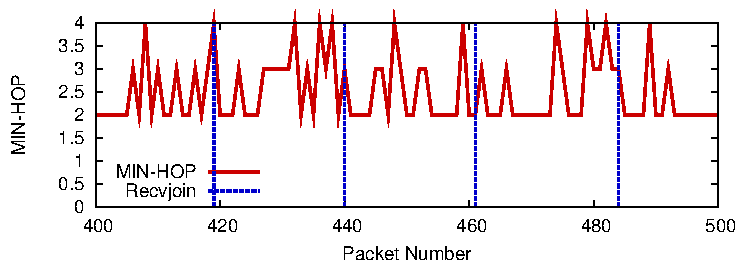
\includegraphics[width=0.4\hsize]{resources/tinyadmr-techrept05/figures/lessons/timeline/Tracecosthop.pdf}
      \\
      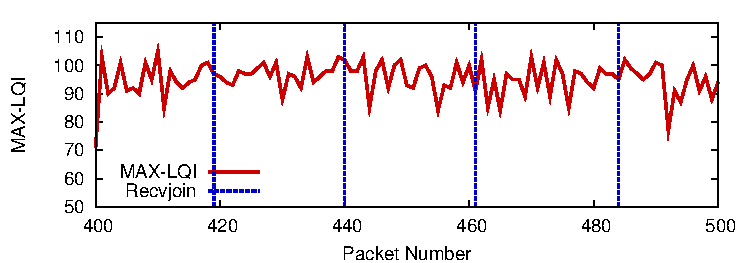
\includegraphics[width=0.4\hsize]{resources/tinyadmr-techrept05/figures/lessons/timeline/Tracecostlqi.pdf}
      \\
      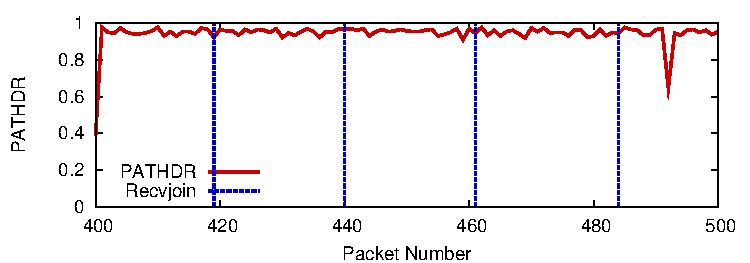
\includegraphics[width=0.4\hsize]{resources/tinyadmr-techrept05/figures/lessons/timeline/Tracecostdr.pdf}
    \end{tabular}
  \end{center}
  \caption{{\small {\bf Stability of path selection metrics over
  time.} {\em This figure plots the value of each of the three
path selection metrics for 100 contiguous data packets for a
single sender-receiver pair. The vertical lines indicate times when 
RECEIVER-JOIN messages were transmitted by the receiver.}}}
\label{fig-pathcostwithtime}
\end{figure}

Receivers select routes based on a single measurement of each path,
which is accumulated as a route discovery message flows from the
senders to the receiver. 
We are concerned with the {\em stability} of the path
measurements over time. If we were to observe high variability in 
the routing metric, then selecting a path based on a single 
measurement of its quality may result in suboptimal paths.

Figure~\ref{fig-pathcostwithtime} shows the value of each of the
three routing metrics, measured across 100~contiguous data packets,
for a single sender-receiver pair. Over time, ADMR is adapting the
path chosen for incoming packets; vertical lines in the figure indicate 
when the node responded with RECEIVER-JOIN messages. The path metric
used in this case is MAX-LQI but we have recorded the measured
values for the MIN-HOP and PATH-DR metrics as well. Note that because
multiple forwarders are active, the specific path traversed by each
incoming data message varies. This can be seen in the MIN-HOP graph 
which shows that the number of hops varies on a per-packet basis.

As the figure shows, the PATH-DR metric is very stable, despite the
different paths traversed by incoming data packets.  MAX-LQI and MIN-HOP
are more variable, suggesting that they are less reliable as a
predictor of overall routing cost.

\subsubsection{The ETX metric}

Another metric 
that has been proposed for choosing good ad-hoc routing paths is the 
{\em minimum expected transmission count} metric~\cite{awoo-multihop}, 
also called ETX~\cite{etx}. ETX is defined as
\[
  p^\star = \arg \min_{p \in P} \sum_{l \in L_p} 
  \frac{1}{\mathrm{LDR}_f(l) \times \mathrm{LDR}_r(l)}
\]
Where $\mathrm{LDR}_f(l)$ and $\mathrm{LDR}_r(l)$ are the 
forward and reverse LDRs for link $l$, respectively.
ETX is intended to maximize path {\em throughput}, rather than
delivery ratio. It is intended primarily for routing protocols
that perform link-by-link acknowledgment and retransmission,
which is why the reverse LDR factors in.

We chose not to implement ETX for two reasons. First, in a multicast
routing protocol such as ADMR, link-layer acknowledgments are 
unnecessary. A forwarder simply rebroadcasts each message it receives, 
which may be received by multiple forwarders or receivers. Unless
some form of multi-receiver acknowledgment were implemented in the
MAC (a feature not currently available in TinyOS radio stack), it is 
not possible to use link-layer acknowledgments in any case. Therefore,
ADMR does not particularly care about the reverse LDR.  The one case
where reverse LDR may affect performance is when propagating
route reply messages, which traverse the reverse path. In our
implementation, link-layer acknowledgment and retransmission are
used only for this message type.

The second reason to avoid ETX is that it relies on a direct
measurement of each link's LDR. While this information can be
gathered by message snooping on regular traffic, a link that 
has never been measured will require multiple rounds of message
exchange to yield an LDR estimate. It is far simpler
and more efficient to use the LQI-based model to predict LDR
as described above.






\subsection{Impact of limited bandwidth}

\begin{figure}[t]
\begin{center}
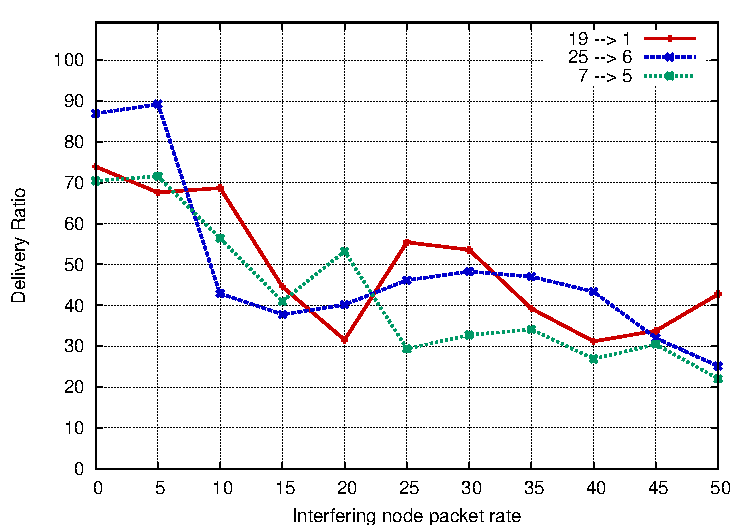
\includegraphics[width=0.6\hsize]{resources/tinyadmr-techrept05/figures/lessons/lesson4/lesson4.pdf}
\end{center}
\caption{{\small {\bf Delivery ratio for three representative paths as
the amount of background traffic is increased.} {\em
Delivery ratio degrades with background traffic despite no
drops by transmitters.}}}
\label{fig-trl}
\end{figure}

Another shortcoming of most MANET protocol designs is that they assume
relatively high link bandwidths. The original ADMR protocol was
evaluated using a simulated 802.11 network with a raw transmission
rate of 2~Mbps. MAC overhead leaves roughly 1~Mbps to applications. 
In contrast, 802.15.4-based radios provide substantially
less capacity. While 802.15.4 operates at a nominal transmission rate
of~250~Kbps, our measurements of the CC2420 using the default radio
stack in TinyOS results in an application data rate of just 25~Kbps with
small packets (28~bytes) and up to 60~Kbps for larger packets
(100~bytes). This is 17~times less than 802.11 at 2~Mbps (1~Mbps for
applications), or 93~times less than 802.11b operating at 11~Mbps 
(5.5~Mbps for applications).

For these reasons we expect protocol overheads to have a serious impact
on the performance of ADMR on 802.15.4. We have not attempted to 
minimize these overheads; rather, our goal is to demonstrate the
practical implications of limited channel bandwidth.

Protocol overhead in ADMR arises primarily due to 
route discovery and route reply messages. In sender-initiated
discovery, each sender periodically floods the network, which 
allows node tables to be maintained on each intermediate node.
When a receiver wishes to establish a path it sends a route reply
back to each sender. The periodic per-sender floods induce the
highest overhead in ADMR and unfortunately scale with network size.
For example, in a network of 30~nodes propagating
per-node floods every 5~sec, the per-node protocol overhead is
$30^2 / 5 = 180$ packets/sec.

Because the size of our testbed is limited, we cannot generate an
arbitrary amount of protocol overhead (which might be seen in a
much larger network) directly. Instead, we cause all nodes in the 
network to generate {\em interference} packets at a rate that we 
control. We then show the impact on the achieved delivery ratio 
for several paths as this interference rate varies.

Figure~\ref{fig-trl} shows the results of this experiment with the per
interfering node interference rate increasing from 0 to 50
packets/sec.  To eliminate effects where a node drops its own
transmissions because it is also generating interference messages,
whenever a node is configured as a forwarder, it generates no
interference messages of its own. While this is not entirely realistic
(a node will still propagate discovery floods while it is acting as a
forwarder), we wanted to avoid losing data transmissions due to queue
overflow on the transmitter.


As the figure shows, the path delivery ratio drops rapidly 
with even a modest amount of background traffic. Keep in mind
that this is {\em not} because forwarders are dropping 
outgoing packets (due to MAC back-off or queue overflow). The only
explanation is that nodes are unable to {\em receive}
packets as well in the presence of interfering traffic. 
That is, the background traffic ``jams'' receivers along the 
ADMR path and prevents them from correctly decoding incoming messages. 
This is likely due to collisions caused by hidden terminal and capture effects. 

We have performed extensive measurements of this 
phenomenon on our testbed and have observed that the LQI and RSSI for
properly received messages is not diminished by the presence 
of background traffic. However, this may be due to the fact that
RSSI and LQI are sampled at the beginning of an incoming message,
while a collision could corrupt the message later during its reception.

\subsection{Impact of route pruning}
\label{sec-tinyadmr-pruning}

\begin{figure}[t]
\begin{center}
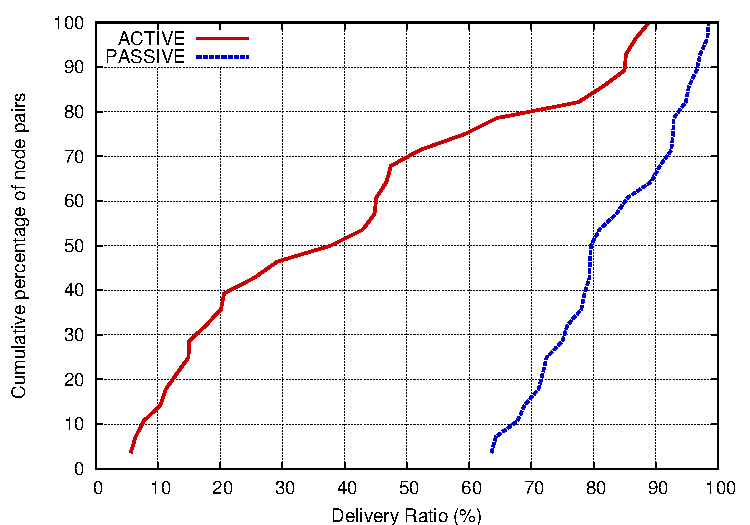
\includegraphics[width=0.6\hsize]{resources/tinyadmr-techrept05/figures/lessons/activevspassive/active_passive.pdf}
\end{center}
\caption{{\small {\bf Comparison of delivery ratio for active vs.
passive route reinforcement.} {\em The MAX-LQI metric is used for this
experiment. With active reinforcement, forwarders are deactivated
more rapidly, which negatively impacts the achieved delivery
ratio.}}}
\label{fig-pruning-cdf}
\end{figure}


\begin{figure}[t]
\begin{center}
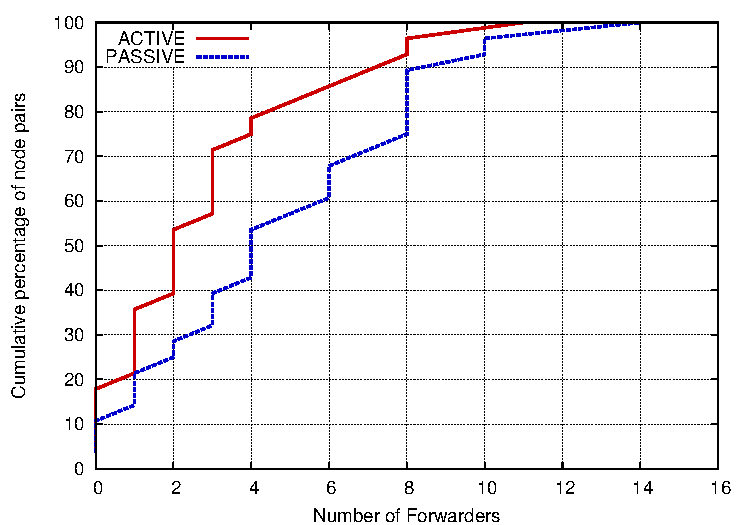
\includegraphics[width=0.6\hsize]{resources/tinyadmr-techrept05/figures/lessons/activevspassive/active_passive_fwd.pdf}
\end{center}
\caption{{\small {\bf Number of active forwarders for active
vs. passive route reinforcement.} 
{\em The number of forwarders is measured at the end of the run,
after pruning has occurred. Active reinforcement only
results in about 2~fewer forwarders.}}}
\label{fig-pruning-forwarders}
\end{figure}



In ADMR, nodes are configured as routers when they receive
a route reply message from a receiver. Over time, different
routes may be activated as link conditions change. Also,
at any given time, multiple routes may exist between 
a single pair of nodes. By pruning redundant routes from
the network over time, communication overheads can be
reduced, although this may also have a negative impact 
on path reliability.

We investigate the impact of two approaches to path pruning in ADMR. The
first, {\em active reinforcement}, requires that nodes continue to
receive route reply messages from a receiver in order to stay active
as forwarders. If a node has not received a route reply for 
10~sec, it clears its forwarder status. This time is equivalent to 
2~discovery cycles. The second approach, {\em passive reinforcement}, 
causes a node to remain active as a forwarder as long as it overhears 
another node retransmitting its own messages (or it continues to 
receive route replies).

Figure~\ref{fig-pruning-cdf} compares the delivery ratio for
the active and passive reinforcement schemes. Not surprisingly, passive
reinforcement keeps more forwarders active, resulting in much higher
reliability than active reinforcement. 
Figure~\ref{fig-pruning-forwarders} shows the number of
forwarders for each of the 28~node pairs at the end of each
100~sec run. Active reinforcement results in about 2~fewer 
forwarders than passive reinforcement. This suggests 
that a small number of additional forwarders can yield a great deal 
of increased reliability.

\subsection{Impact of limited node state}
\label{sec-tinyadmr-node-state}

The final lesson that we explore involves the impact of limited
node state. Sensor nodes such as the Telos and MicaZ have 
notoriously small memory sizes: the MSP430 microprocessor
has only 10~KB of RAM, while the Atmega 128L has just 4~KB. 
We cannot expect that the routing layer can consume an arbitrary 
amount of memory to store its routing state. This is especially
true if there is a substantial application running on top of
the routing layer that has its own memory requirements.

The node table maintained by every ADMR node potentially
contains one entry for every other node in the network.
In our implementation, each entry consumes 8~bytes.
In a very large network, it is clear that the number of
entries in this table can quickly saturate memory.

The original ADMR paper~\cite{admr} suggests using an LRU
strategy to prune node table entries over time. However, 
in a network with many active senders it may not be possible
to guarantee an upper bound on the node table size. 
We are concerned with how to deal with {\em overflow} in the node 
table given some fixed limit on its size. 

Upon receipt of a discovery message, ADMR will consult the node 
table and either update the existing entry for this sender, or
attempt to create a new entry. If the table is full, we must either
drop the new entry or evict some other entry to make room.
Dropping a node table entry has two effects. The first is that the node
loses information on the routing cost from the sender. This is
only needed when establishing new routes, so these entries
are only needed shortly after a discovery message has been
received (in case the receiver wishes to reinforce this route).

The second effect is that the last sequence number received
from this node, used for duplicate suppression, is lost. 
This information is required for all senders for which this
node is a forwarder. This suggests that ADMR should keep
the last sequence number and reverse-path information in 
separate tables, although this is not the case in the
original protocol design.

We explore several different policies for evicting table entries.
The most naive policy simply drops the new entry if the table is full,
only allowing updates to entries already in the table. 
Another simple policy is FIFO, which drops the oldest entry 
(where entries are ordered by time of insertion). FIFO is intended to 
time out stale entries from the table in favor of new entries. However,
if the routing cost for the new entry is very high, it may not
be worthwhile maintaining information on this route. 

A better approach may be to maintain node table entries for 
high-quality routes, with the expectation that this node will
be called upon to act as a forwarder. In some sense, the impact
of dropping discovery messages for low-quality paths should not
be too severe. 

Figure~\ref{fig-routing-table-management} shows a comparison 
of each of these table-management policies with 6~senders and
1~receiver. We emulate the impact of a large network by artificially
limiting the node table size to 4~entries on each node. 
This implies that nodes will not be able to maintain routing state for 
all 6~senders. As the results show, none of the proposed 
policies works well in all cases. The naive drop-new-entry
policy performs very poorly. The FIFO and drop-worst policies 
work reasonably for only 3 out of the 6 routes. Since there are always some
routes that are hurt badly by evicting entries in node tables, it suggests
that approaches that avoid discarding information from node tables are
desired.

One potential solution to managing limited memory size is to swap node 
table entries to external memory (such as flash) on demand. We have not
yet explored this approach, although the results presented above
suggest it may be necessary to do so in large networks.

\begin{figure}[t]
\begin{center}
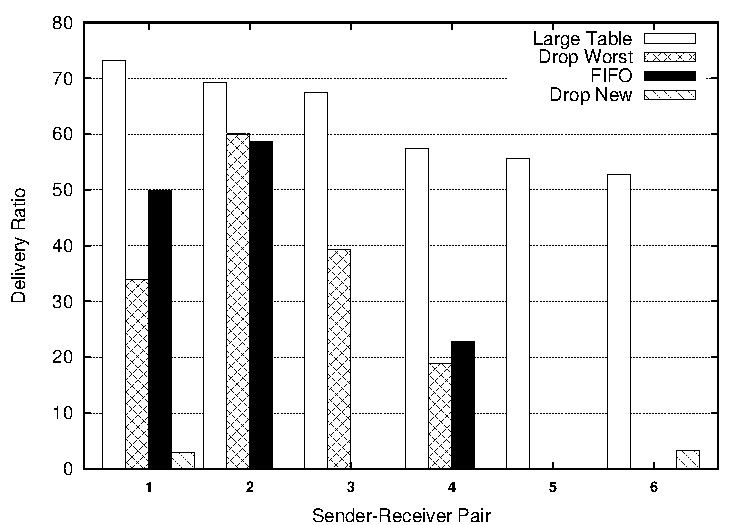
\includegraphics[width=0.6\hsize]{resources/tinyadmr-techrept05/figures/lessons/tablesize/limited_table_size.pdf}
\end{center}
\caption{{\small {\bf Comparison of delivery performance 
with different node table management strategies.}
{\em This experiment uses 6 senders and 1 receiver.
In each case except for {\em Large Table},
the node table size is limited to~4~entries
to simulate the effect of scaling in a large network.
None of the proposed schemes for prioritizing node
table entries works well in all cases.}}}
\label{fig-routing-table-management}
\end{figure}

\section{Design considerations and discussion}


TinyADMR is intended to support publish/subscribe routing in our prototype of
CodeBlue architecture. However, our current implementation is not the only way
to realize CodeBlue's routing layer, nor is it optimal for all applications.
Although TinyADMR can be used by different applications, many of our design
decisions are motivated by the goal to support our target application domain:
patient vital sign monitoring in disaster response scenarios. In the following
sections, we describe our important design choices, lessons, and potential future
improvements for efficient and scalable multicast routing on
mote-based sensor networks.

\subsection{Ad-hoc multicast routing protocols}

Since there are existing multicast routing protocols designed by the MANET
research community~\cite{admr, maodv, odmrp}, we chose to use an existing
protocol instead of designing a new one from the ground up. We compared
three on-demand multicast routing protocols according to their published
simulation studies. These three protocols are: ADMR, ODMRP, and MAODV.
Jetcheva et al.~\cite{admr} compared ADMR and ODMRP directly and showed that both
protocols achieve high delivery ratio when the nodes in the network are
stationary. However, ODMRP's performance degrades faster than ADMR as the
mobility level of the network increases. In addition, ADMR incurs lower
protocol overhead and achieves lower latency than ODMRP. 

Unlike ADMR and ODMRP, MAODV's multicast group does not distinguish senders
versus receivers. Therefore, all nodes belonging to a multicast group will
receive data packets sent to this address. This model creates redundant
traffic because members of the multicast group that only send packets do not
need to receive packets from each other. Especially in CodeBlue scenarios, it
is likely that there will always be more sending devices (patients) than
receiving devices (doctors) in any multicast group. In this case, MAODV will
forward data to not only receiving devices held by doctors but also other
patient devices, which is unnecessary and a waste of already limited bandwidth
capacity. Moreover, comparing the data in ADMR study~\cite{admr} and MAODV
simulation data by Royer et al.~\cite{maodv} indicates that ADMR achieves
higher delivery performance even when the nodes in the ADMR simulations are
moving at higher speed than in MAODV simulations.

For above reasons, we chose ADMR, among the three candidate
protocols, to be the protocol that implements publish/subscribe layer in
CodeBlue. 

\subsection{Realistic wireless link conditions}

One major contribution made by our TinyADMR study is proposing the use of link
quality aware routing metrics, PATH-DR and MAX-LQI. This is a lesson that we
learned through the use of a real testbed. One potential caveat 
is that this is derived from the link conditions of our particular testbed and
may not apply to other situations where there are fewer low quality links.
However, since we are targeting at patient vital sign monitoring application,
there are likely to be many low quality and asymmetric links.  Our experience
shows that the radio link quality and asymmetry depend on many factors,
including variation in antenna sensitivity, distance between nodes, and
obstructive objects (e.g. floors, walls, doors, and human body). Since nodes
are worn by patients, their bodies will be obstructing the radio wave.
Consequently, low quality and asymmetric links will exist for most of the
patient nodes in our target scenario. Therefore, the routing protocol must try
to avoid these low quality links in order to achieve good delivery performance
and that is why we believe replacing MIN-HOP with link quality based routing
metric such as PATH-DR is necessary. In fact, avoiding the use of MIN-HOP is
necessary also because it is likely to {\em prefer} low quality links over
high quality ones. The reason is that a shortest hop count path often involves
links over longer physical distance and they tend to have worse
quality because radio signal strength decays more over longer distances. Due
to the above reasons, we decided that it is necessary to take link quality
into account when choosing routes for our application scenarios.

\subsection{Routing table management}

Scalability limitation of ADMR due to memory constraint
is one of the most difficult challenges for applying it in large deployments.
For our experiments, we could afford to devote enough memory space to support
networks of up to 30 nodes. Given limited time to finish the complete system
for CodeBlue deployment study, we were only able to explore several simple
policies for managing the node table
(Section~\ref{sec-tinyadmr-node-state}), trying to address the scalability
issue. Our attempt to resolve the memory limitation issue was not very
successful. However, we would like to point out that several additional
improvements can
potentially address the scalability issue for larger networks. 

As analyzed in Section~\ref{sec-tinyadmr-node-state}, the scale of an ADMR
network is limited by the size of node table. With the current design, node
table serves two purposes: route discovery and duplicate rejection. Route
discovery is enabled by storing sender address (2 bytes), path cost (2 bytes)
and the previous hop address (2 bytes) in node table. Duplicate rejection is
enabled by remembering the last seen sequence number (2 bytes) for each sender
in the network. Therefore, an entry in the node table occupies 8 bytes.

Route discovery related fields in the node table are needed to set up the
forwarders for each multicast group. These fields are needed during the
process of route discovery. Remembering sequence numbers for duplicate
suppression is essential to support correct flooding of route discovery packets
because it is the information that a node uses to decide whether an incoming
packet is newly seen or not. Each node only re-broadcasts an incoming packet
if its sequence number is considered new. This mechanism is important because
otherwise any flooded packet would be retransmitted by all nodes indefinitely. 
The sequence number also determines whether a packet should be
passed to the application layer. Therefore, sequence numbers are
important to be stored and updated over the course of the network
lifetime to ensure correct packet delivery.

Given above observation, it is possible to reclaim much of the space
used by node table by splitting it into two tables: route discovery
table and sequence number table. Notice that each entry in a route discovery table 
is needed only during the relevant route discovery session, which typically
takes no more than a few seconds to complete. Therefore, it would be enough
to keep each entry in route discovery table for only a short
period of time (e.g. 10 seconds) because the information will not be needed
once the route has been set up. The current structure of node table does not
allow this because sequence numbers are stored in the same table as route
discovery information. 
With the new two-table arrangement, the discovery table
size does not limit the total number of publishing nodes anymore. Instead, it only
limits the maximal amount of {\em concurrent} route discovery sessions in the
network. Number of concurrent route discovery sessions can be minimized by staggering
the route discovery time for each publishing nodes. One simple way to do this
is to add a random delay to route discovery timer each time it fires. 

It is also possible to further optimize the space used by the proposed
sequence number table. Even though it is important to remember sequence
numbers for each sender in the network in order to tell which incoming packets
are new, such information does not have to be stored as a table that grows
proportionally with the the number of nodes it needs to remember. For example,
it is possible to use smarter data structures such as a Bloom filter to store
the sender id and the sequence number of flooded packets that are received.
This Bloom filter can then be used to perform duplicate suppression for
checking whether rebroadcasting an incoming packet is needed. As long as the
false positive rate is low enough, the Bloom filter approach will only need a
constant memory space to implement the duplicate rejection mechanism with a
low probability of sacrificing correctness. Alternatively, simply applying
compression to the sequence number table can also significantly save the
memory consumed by this table and increase the scalability of the protocol.


\section{Summary}
\label{sec-tinyadmr-future}
\label{sec-tinyadmr-futurework}
\label{sec-tinyadmr-conclusions}
\label{sec-tinyadmr-conclusion}

In this chapter, we have investigated many aspects of providing
publish/subscribe abstraction with ADMR multicast routing protocol on
mote-based sensor networks. We have found translating ADMR into real
implementation for a
resource limited platform to be rather challenging, especially when
expecting similar performance as shown in earlier simulation studies. Specifically, we 
found that the original design of ADMR performs poorly on our real testbed
because of the use of MIN-HOP as its route selection metric. We found that, in a realistic
environment, MIN-HOP often leads to the choice of routing paths with low
packet delivery performance. To address this problem, we proposed and
evaluated two new routing metrics: MAX-LQI and PATH-DR. The two new metrics
both perform significantly better than MIN-HOP on our testbed. One important
contribution of these two new metrics is that we obtain
link quality data by leveraging the link estimation process from the
physical layer and therefore do not incur additional measurement overhead, as
required by earlier work ETX~\cite{etx} and MintRoute~\cite{awoo-multihop}.

We have studied scalability limitations of ADMR when implemented on
motes. We found that the flooding of route discovery messages to have negative
impact on the packet delivery performance as the network scales up. 
Memory constraint on the mote platform is another
limiting factor of ADMR scalability. The reason is that the routing table size
must grow with the network size in order for the protocol to correctly
establish routing paths. To address this problem, we have conducted experiments with different table eviction policies based
on FIFO, LIFO, and drop-worst rules but none of the above policy
worked without sacrificing routing performance significantly.

With our experimental results, we show that TinyADMR is practical for
providing publish/subscribe routing in real sensor networks but the network
scale is limited by protocol overhead and available memory space. 
After identifying the reason of the memory limitation, we also describe a
potential strategy to remove the memory limitation in future systems by
changing the routing table structure and expiring unnecessary routing state
frequently.
